% =====================================================================
%  Slide thuyet trinh - He thong sinh cau hoi trac nghiem Toan da tac tu
%
%  Bien dich:  xelatex SlideThuyetTrinh.tex   (chay 2 lan de co so trang)
%  Hinh ve:    ../figs/
%
%  GHI CHU NGUOI NOI: phan dien giai nam trong cac khoi \note{...}.
%  - Mac dinh: KHONG in ra (slide sach, it chu).
%  - Muon xem: bo dau % o dong \setbeameroption ben duoi.
% =====================================================================
\documentclass[aspectratio=169,11pt]{beamer}

% \setbeameroption{show notes}                    % in slide + trang ghi chu xen ke
% \setbeameroption{show notes on second screen}   % trinh chieu 2 man hinh

% ------------------------- Font & ngon ngu --------------------------
\usepackage{fontspec}
\setsansfont{texgyreheros}[
  Extension      = .otf,
  UprightFont    = *-regular,
  BoldFont       = *-bold,
  ItalicFont     = *-italic,
  BoldItalicFont = *-bolditalic ]
\setmonofont{texgyrecursor}[
  Extension   = .otf,
  UprightFont = *-regular,
  BoldFont    = *-bold ]
\usepackage[vietnamese]{babel}

% ------------------------------ Goi -------------------------------
\usepackage{graphicx}
\usepackage{booktabs}
\usepackage{array}
\usepackage{tikz}
\usetikzlibrary{arrows.meta, positioning}
\usepackage{amsmath, amssymb}

% ----------------------------- Giao dien ----------------------------
\usetheme{default}
\usefonttheme{professionalfonts}
\setbeamertemplate{navigation symbols}{}

\definecolor{cPrimary}{HTML}{1F3A5C}   % xanh dam
\definecolor{cAccent} {HTML}{C1440E}   % cam gach
\definecolor{cDet}    {HTML}{1B7F5C}   % xanh la - tat dinh
\definecolor{cMuted}  {HTML}{6B7280}   % xam
\definecolor{cBg}     {HTML}{F4F5F7}

\setbeamercolor{structure}{fg=cPrimary}
\setbeamercolor{frametitle}{fg=white, bg=cPrimary}
\setbeamercolor{title}{fg=cPrimary}
\setbeamercolor{alerted text}{fg=cAccent}
\setbeamercolor{block title}{fg=white, bg=cPrimary}
\setbeamercolor{block body}{bg=cBg}
\setbeamercolor{block title alerted}{fg=white, bg=cAccent}
\setbeamercolor{block body alerted}{bg=cBg}
\setbeamercolor{itemize item}{fg=cAccent}

\setbeamertemplate{itemize item}{\raisebox{0.15ex}{\tiny$\blacksquare$}}
\setbeamertemplate{blocks}[rounded][shadow=false]

\setbeamertemplate{frametitle}{%
  \nointerlineskip
  \begin{beamercolorbox}[wd=\paperwidth, ht=2.9ex, dp=1.3ex, leftskip=0.8em, rightskip=0.8em]{frametitle}
    \usebeamerfont{frametitle}\strut\insertframetitle\hfill
    {\footnotesize\color{white!75!cPrimary}\insertsectionhead}
  \end{beamercolorbox}
}
\setbeamerfont{frametitle}{size=\large, series=\bfseries}
\setbeamerfont{block title}{size=\normalsize, series=\bfseries}
\setbeamerfont{footline}{size=\tiny}

\setbeamertemplate{footline}{%
  \hbox{\begin{beamercolorbox}[wd=\paperwidth, ht=2.4ex, dp=1ex, leftskip=0.8em, rightskip=0.8em]{}
    \color{cMuted}\tiny Hệ thống AQG Toán đa tác tử\hfill\insertframenumber/\inserttotalframenumber
  \end{beamercolorbox}}
}

\setbeamerfont{note page}{size=\small}

% ----------------------------- Lenh tat ------------------------------
\newcommand{\dt}[1]{\textcolor{cDet}{\textbf{#1}}}
\renewcommand{\cite}[1]{\textcolor{cMuted}{[#1]}}
% Dong nguon nho cuoi slide
\newcommand{\srcnote}[1]{\vfill{\scriptsize\color{cMuted}#1\par}}
% Cau chot giua slide
\newcommand{\punch}[1]{\begin{center}\alert{\large #1}\end{center}}
% Huy hieu danh dau ky thuat tu de xuat -- dung trong tieu de slide
\newcommand{\dg}{\;\raisebox{0.15ex}{\colorbox{cAccent}{\color{white}\scriptsize\bfseries\,ĐÓNG GÓP\,}}}
% Khoi noi bat cho ky thuat tu de xuat
\newcommand{\dgtag}{{\scriptsize\color{cAccent}$\blacklozenge$\,\textbf{Đóng góp}}\ }

% ------------------------------ Tieu de ------------------------------
\title{\bfseries Hệ thống sinh câu hỏi trắc nghiệm Toán\\đa tác tử có kiểm chứng và phản hồi người dùng}
\subtitle{Phương pháp, kiến trúc và kỹ thuật}
\author{}
\date{}

\begin{document}

% =====================================================================
\begin{frame}[plain]
  \titlepage
  \vspace{-2em}
  \centering
  {\footnotesize\color{cMuted}Báo cáo kỹ thuật --- trình bày tóm tắt}
\end{frame}

% =====================================================================
\begin{frame}{Nội dung}
  \vfill
  \begin{columns}[T]
    \begin{column}{0.5\textwidth}
      \begin{enumerate}
        \item Bài toán
        \item Kiến trúc
        \item Các kỹ thuật chính
        \item Kiểm soát chất lượng
      \end{enumerate}
    \end{column}
    \begin{column}{0.5\textwidth}
      \begin{enumerate}
        \setcounter{enumi}{4}
        \item Phản hồi người dùng
        \item Ngân hàng câu hỏi
        \item Đối chiếu nghiên cứu
        \item Hướng phát triển
      \end{enumerate}
    \end{column}
  \end{columns}
  \vfill
  \punch{Toán có đáp án kiểm chứng được bằng máy.\\[0.2em] Hệ thống dùng tính chất đó làm \textbf{tài sản kiến trúc}.}
  \vfill
  \note{
    Luận điểm trung tâm của cả bài: khác với sinh câu hỏi đọc hiểu, một câu hỏi Toán có đáp án đúng/sai xác định được bằng máy. Hầu hết các hệ AQG hiện nay phó thác việc thẩm định cho chính mô hình ngôn ngữ. Hệ thống này thì không --- nó khai thác tính kiểm chứng được như một thành phần kiến trúc.
  }
\end{frame}

% =====================================================================
\begin{frame}{Sáu đóng góp của hệ thống}
  \vspace{0.2em}
  \begin{center}
    \small Sáu kỹ thuật dưới đây do hệ thống \textbf{tự đề xuất}. Chúng sẽ được đánh dấu \dg\ khi xuất hiện.
  \end{center}
  \vspace{0.4em}
  \begin{columns}[T]
    \begin{column}{0.5\textwidth}
      \begin{alertblock}{Nhóm 1 --- Khai thác tầng kiểm chứng}
        \small
        \begin{enumerate}
          \item \textbf{Loại trừ đa đáp án} bằng kiểm chứng ký hiệu trên chính các nhiễu
          \smallskip
          \item \textbf{Tự sửa đáp án} từ nhiễu được kiểm chứng
          \smallskip
          \item Chính sách \textbf{``không khớp $\neq$ sai''}
        \end{enumerate}
      \end{alertblock}
    \end{column}
    \begin{column}{0.5\textwidth}
      \begin{alertblock}{Nhóm 2 --- Biến chủ quan thành kiểm chứng được}
        \small
        \begin{enumerate}
          \setcounter{enumi}{3}
          \item \textbf{Mô tả lỗi phải dẫn ra đúng giá trị} phương án nhiễu
          \smallskip
          \item \textbf{Kiểm soát độ khó hai trục}
          \smallskip
          \item \textbf{Lập lịch least-covered-first có bù hụt} dưới điều kiện song song
        \end{enumerate}
      \end{alertblock}
    \end{column}
  \end{columns}
  \vfill
  \punch{Cả sáu đều bắt nguồn từ \emph{một} lựa chọn kiến trúc:\\[0.2em] đưa tính kiểm chứng được vào lõi hệ thống.}
  \vfill
  \note{
    Slide này là bản đồ cho cả phần sau. Sáu kỹ thuật này không tìm thấy tương đương trong phạm vi các tài liệu được cung cấp --- em trình bày chúng như đóng góp của hệ thống.

    Cách chia nhóm cũng có ý: nhóm 1 là những gì mở ra được khi đã có tầng kiểm chứng tất định; nhóm 2 là nguyên tắc biến phẩm chất chủ quan thành mệnh đề máy kiểm được.

    Mỗi kỹ thuật sẽ được đánh dấu bằng huy hiệu ĐÓNG GÓP trên tiêu đề slide khi nó xuất hiện, để thầy cô dễ theo dõi.

    Nếu buổi trình bày bị rút ngắn, đây là slide không được bỏ.
  }
\end{frame}

% =====================================================================
\section{Bài toán}
\begin{frame}{Ba yêu cầu đặc thù}
  \vfill
  \begin{columns}[T]
    \begin{column}{0.33\textwidth}
      \begin{block}{1. Bám tài liệu}
        Câu hỏi từ tài liệu của giảng viên --- không từ tri thức nền của mô hình.
      \end{block}
    \end{column}
    \begin{column}{0.33\textwidth}
      \begin{block}{2. Đúng toán học}
        Đáp án phải được \alert{máy tính lại}.
      \end{block}
    \end{column}
    \begin{column}{0.33\textwidth}
      \begin{block}{3. Đo lường được}
        Mỗi câu gắn một mức Bloom và một chuẩn đầu ra.
      \end{block}
    \end{column}
  \end{columns}
  \vfill
  \punch{Hai điểm nghẽn cố hữu của AQG:\\[0.2em] \textbf{chất lượng} và \textbf{khả năng kiểm soát}.}
  \vfill
  \srcnote{\cite{17}, \cite{18} --- khảo sát sinh câu hỏi và sinh phương án nhiễu.}
  \note{
    Ba yêu cầu này vượt ra ngoài phạm vi của các hệ AQG dựa trên văn bản thông thường.

    Yêu cầu 2 là điểm mấu chốt: khác với sinh câu hỏi đọc hiểu, câu hỏi Toán kiểm chứng được bằng máy --- hệ thống phải khai thác tính chất này.

    Yêu cầu 3 nhằm để bộ câu hỏi thu được là một công cụ đo lường có cấu trúc, chứ không phải một tập câu hỏi rời rạc.

    Hai điểm nghẽn nêu ở dưới được ghi nhận trong cả hai bài khảo sát. Toàn bộ thiết kế được tổ chức xoay quanh chính hai điểm nghẽn này.
  }
\end{frame}

% =====================================================================
\begin{frame}{Đầu vào và đầu ra}
  \vfill
  \begin{columns}[T]
    \begin{column}{0.42\textwidth}
      \begin{block}{Vào}
        \begin{itemize}
          \item Tài liệu PDF
          \item Số câu
          \item Phân bố Bloom
          \item Độ khó mục tiêu
          \item Danh sách chuẩn đầu ra
        \end{itemize}
      \end{block}
    \end{column}
    \begin{column}{0.58\textwidth}
      \begin{block}{Ra --- mỗi câu mang theo}
        \begin{itemize}
          \item 3 nhiễu \alert{kèm mô tả lỗi}
          \item Lời giải từng bước
          \item \alert{Trích dẫn nguyên văn} làm bằng chứng
          \item Nhãn Bloom, chuẩn đầu ra, độ khó
          \item Điểm rubric, trạng thái duyệt
        \end{itemize}
      \end{block}
    \end{column}
  \end{columns}
  \vfill
  \srcnote{Kèm theo cả lượt: siêu dữ liệu vận hành và danh sách câu bị loại có mã lý do.}
  \note{
    Đầu vào: một tài liệu học liệu PDF và một cấu hình sinh do người dùng khai báo, kèm tuỳ chọn có lời giải chi tiết hay không.

    Đầu ra: bộ câu hỏi bốn phương án. Hai thứ đáng chú ý ở cột phải --- mỗi phương án nhiễu mang theo mô tả lỗi tương ứng, và mỗi câu mang theo một trích dẫn nguyên văn từ tài liệu. Cả hai đều là dấu vết để kiểm tra lại, sẽ nói kỹ ở phần sau.
  }
\end{frame}

% =====================================================================
\section{Kiến trúc}
\begin{frame}{Năm giai đoạn}
  \vspace{0.5em}
  \begin{center}
    \small
    \begin{tabular}{@{}c l l@{}}
      \toprule
      & \textbf{Nội dung} & \textbf{Bản chất} \\
      \midrule
      \textcircled{\scriptsize 1} & Chuẩn bị tài liệu       & Chạy ngầm, một lần \\
      \textcircled{\scriptsize 2} & Sinh câu hỏi            & \alert{Đa tác tử, song song} \\
      \textcircled{\scriptsize 3} & Hậu xử lý               & Một lần cho cả lượt \\
      \textcircled{\scriptsize 4} & Duyệt                   & \alert{Vòng lặp con người} \\
      \textcircled{\scriptsize 5} & Nhập ngân hàng          & Theo từng câu \\
      \bottomrule
    \end{tabular}
  \end{center}
  \vfill
  \punch{Chuẩn bị chạy ngay khi \emph{chọn} tài liệu ---\\[0.2em] trước khi người dùng cấu hình xong.}
  \vfill
  \note{
    Giai đoạn 1: kiểm định, đóng gói tài liệu, trích dàn ý gợi ý cấu hình.
    Giai đoạn 2: bộ điều phối vận hành chuỗi năm tác tử cho từng câu.
    Giai đoạn 3: kiểm chứng nhãn chuẩn đầu ra, lưu kết quả và nhật ký loại bỏ.
    Giai đoạn 4: người dùng đánh giá, sinh lại, sinh thêm, luyện tập, xuất bản.
    Giai đoạn 5: khử trùng lặp ba tầng rồi nhập kho.

    Câu chốt phía dưới là một quyết định về trải nghiệm nhưng có hệ quả kiến trúc. Nó buộc phần đóng gói tài liệu phải tách rời hoàn toàn khỏi phần cấu hình sinh. Đổi lại, hệ thống dùng chính lượt đọc lướt tài liệu đó để gợi ý ngược cấu hình cho người dùng --- chủ đề, chuẩn đầu ra, số câu hợp lý --- thay vì bắt họ khai báo từ con số không.
  }
\end{frame}

% =====================================================================
\begin{frame}{Kiến trúc tổng thể}
  \vfill
  \begin{center}
    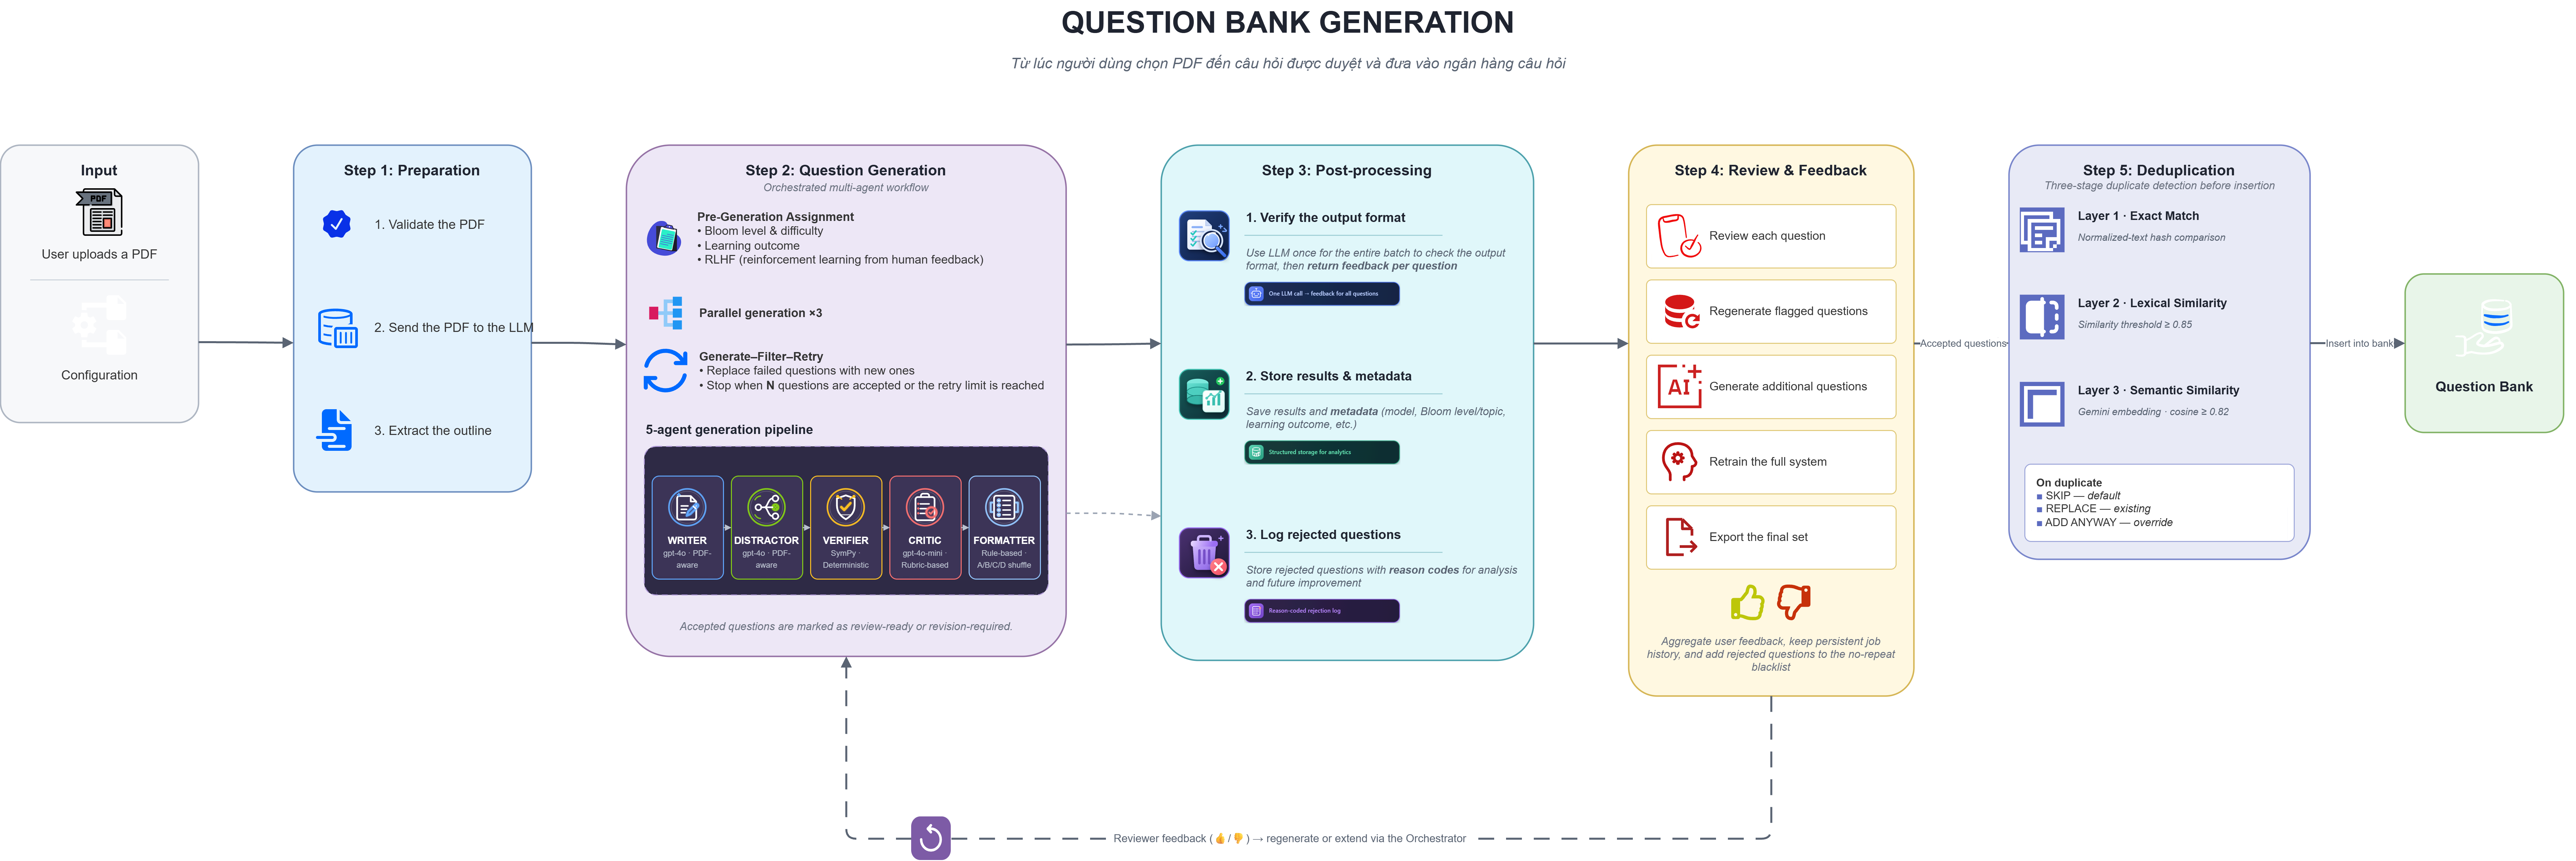
\includegraphics[width=0.98\textwidth]{../figs/pipeline-tong-the.png}
  \end{center}
  \vfill
  \note{
    Tài liệu đi qua năm giai đoạn từ trái sang phải. Chuỗi năm tác tử nằm trong giai đoạn 2 --- dải màu đậm ở giữa.

    Đường nét đứt phía dưới là vòng phản hồi người dùng: đánh giá ở giai đoạn 4 được đưa ngược về bộ điều phối để sinh lại hoặc sinh bổ sung, mà không cần tải lại tài liệu.

    Ba tầng khử trùng lặp ở giai đoạn 5 được xếp theo chi phí tăng dần --- sẽ nói kỹ ở phần ngân hàng câu hỏi.
  }
\end{frame}

% =====================================================================
\begin{frame}{Bộ điều phối}
  \punch{Một mục tiêu duy nhất: thu về đủ $N$ câu đạt chuẩn.}
  \vfill
  \begin{columns}[T]
    \begin{column}{0.33\textwidth}
      \begin{block}{Giao chỉ tiêu trước}
        Bloom, độ khó, chuẩn đầu ra được ấn định \alert{trước} mọi lời gọi mô hình.
      \end{block}
    \end{column}
    \begin{column}{0.33\textwidth}
      \begin{block}{Điều phối song song}
        Sinh đồng thời theo đợt.\\
        Ghép kết quả: tuần tự.
      \end{block}
    \end{column}
    \begin{column}{0.33\textwidth}
      \begin{block}{Quyết định dừng}
        Đủ số câu $\cdot$ vượt hạn mức thử $\cdot$ thất bại liên tiếp.
      \end{block}
    \end{column}
  \end{columns}
  \vfill
  \srcnote{Nó không soạn nội dung câu hỏi, và không tự đánh giá chất lượng.}
  \note{
    Giao chỉ tiêu trước: cách này trái ngược với việc sinh một tập câu hỏi rồi phân loại về sau --- nó biến phân bố mong muốn thành một ràng buộc đầu vào thay vì một kết quả cần hy vọng.

    Điều phối song song: phần ghép kết quả, khử trùng lặp và cập nhật trạng thái được giữ tuần tự để tránh tranh chấp dữ liệu. Bước kiểm chứng ký hiệu cũng được tuần tự hoá riêng do thư viện tính toán ký hiệu không cam kết an toàn đa luồng --- đây là bước thuần CPU và nhanh nên không gây nghẽn.

    Điều kiện dừng: ngưỡng thất bại liên tiếp được đặt tương đối theo số câu yêu cầu, để một mục tiêu lớn không bị dừng sớm chỉ vì gặp một chuỗi lỗi tạm thời từ nhà cung cấp mô hình.
  }
\end{frame}

% =====================================================================
\begin{frame}{Chuỗi năm tác tử --- cho \emph{mỗi} câu}
  \vspace{0.5em}
  \begin{center}
    \small
    \begin{tabular}{@{}c l l@{}}
      \toprule
      \# & \textbf{Tác tử} & \textbf{Nhiệm vụ} \\
      \midrule
      1 & Writer     & Đề, đáp án, lời giải, trích dẫn, biểu thức kiểm chứng \\
      2 & Distractor & Ba phương án nhiễu \\
      3 & \dt{Verifier}  & \dt{Tất định} --- kiểm chứng toán học \\
      4 & Critic     & Chấm bám nguồn và sáu tiêu chí rubric \\
      5 & \dt{Formatter} & \dt{Tất định} --- đóng gói, trộn phương án, phân luồng \\
      \bottomrule
    \end{tabular}
  \end{center}
  \vfill
  \punch{Việc gì máy tính được chính xác\\[0.2em] thì không giao cho mô hình ngôn ngữ.}
  \vfill
  \srcnote{\dt{Hai trên năm} tác tử tất định --- khác các khung đa tác tử thuần LLM \cite{20}, \cite{21}, \cite{24}. \quad Không có tác tử Refiner: xem phần sau.}
  \note{
    Ba tác tử dùng mô hình ngôn ngữ (Writer, Distractor, Critic) đều đọc trực tiếp tài liệu PDF.

    Verifier và Formatter hoàn toàn tất định, không gọi mô hình nào.

    Tỉ lệ hai trên năm tác tử tất định là điểm khác biệt căn bản so với các khung đa tác tử thuần LLM cho sinh câu hỏi trong các bài báo được khảo sát.

    Việc không có tác tử Refiner là một lựa chọn có chủ ý --- sẽ phân tích ở phần kiểm soát chất lượng.
  }
\end{frame}

% =====================================================================
\begin{frame}{Chuỗi tác tử --- chi tiết}
  \vfill
  \begin{center}
    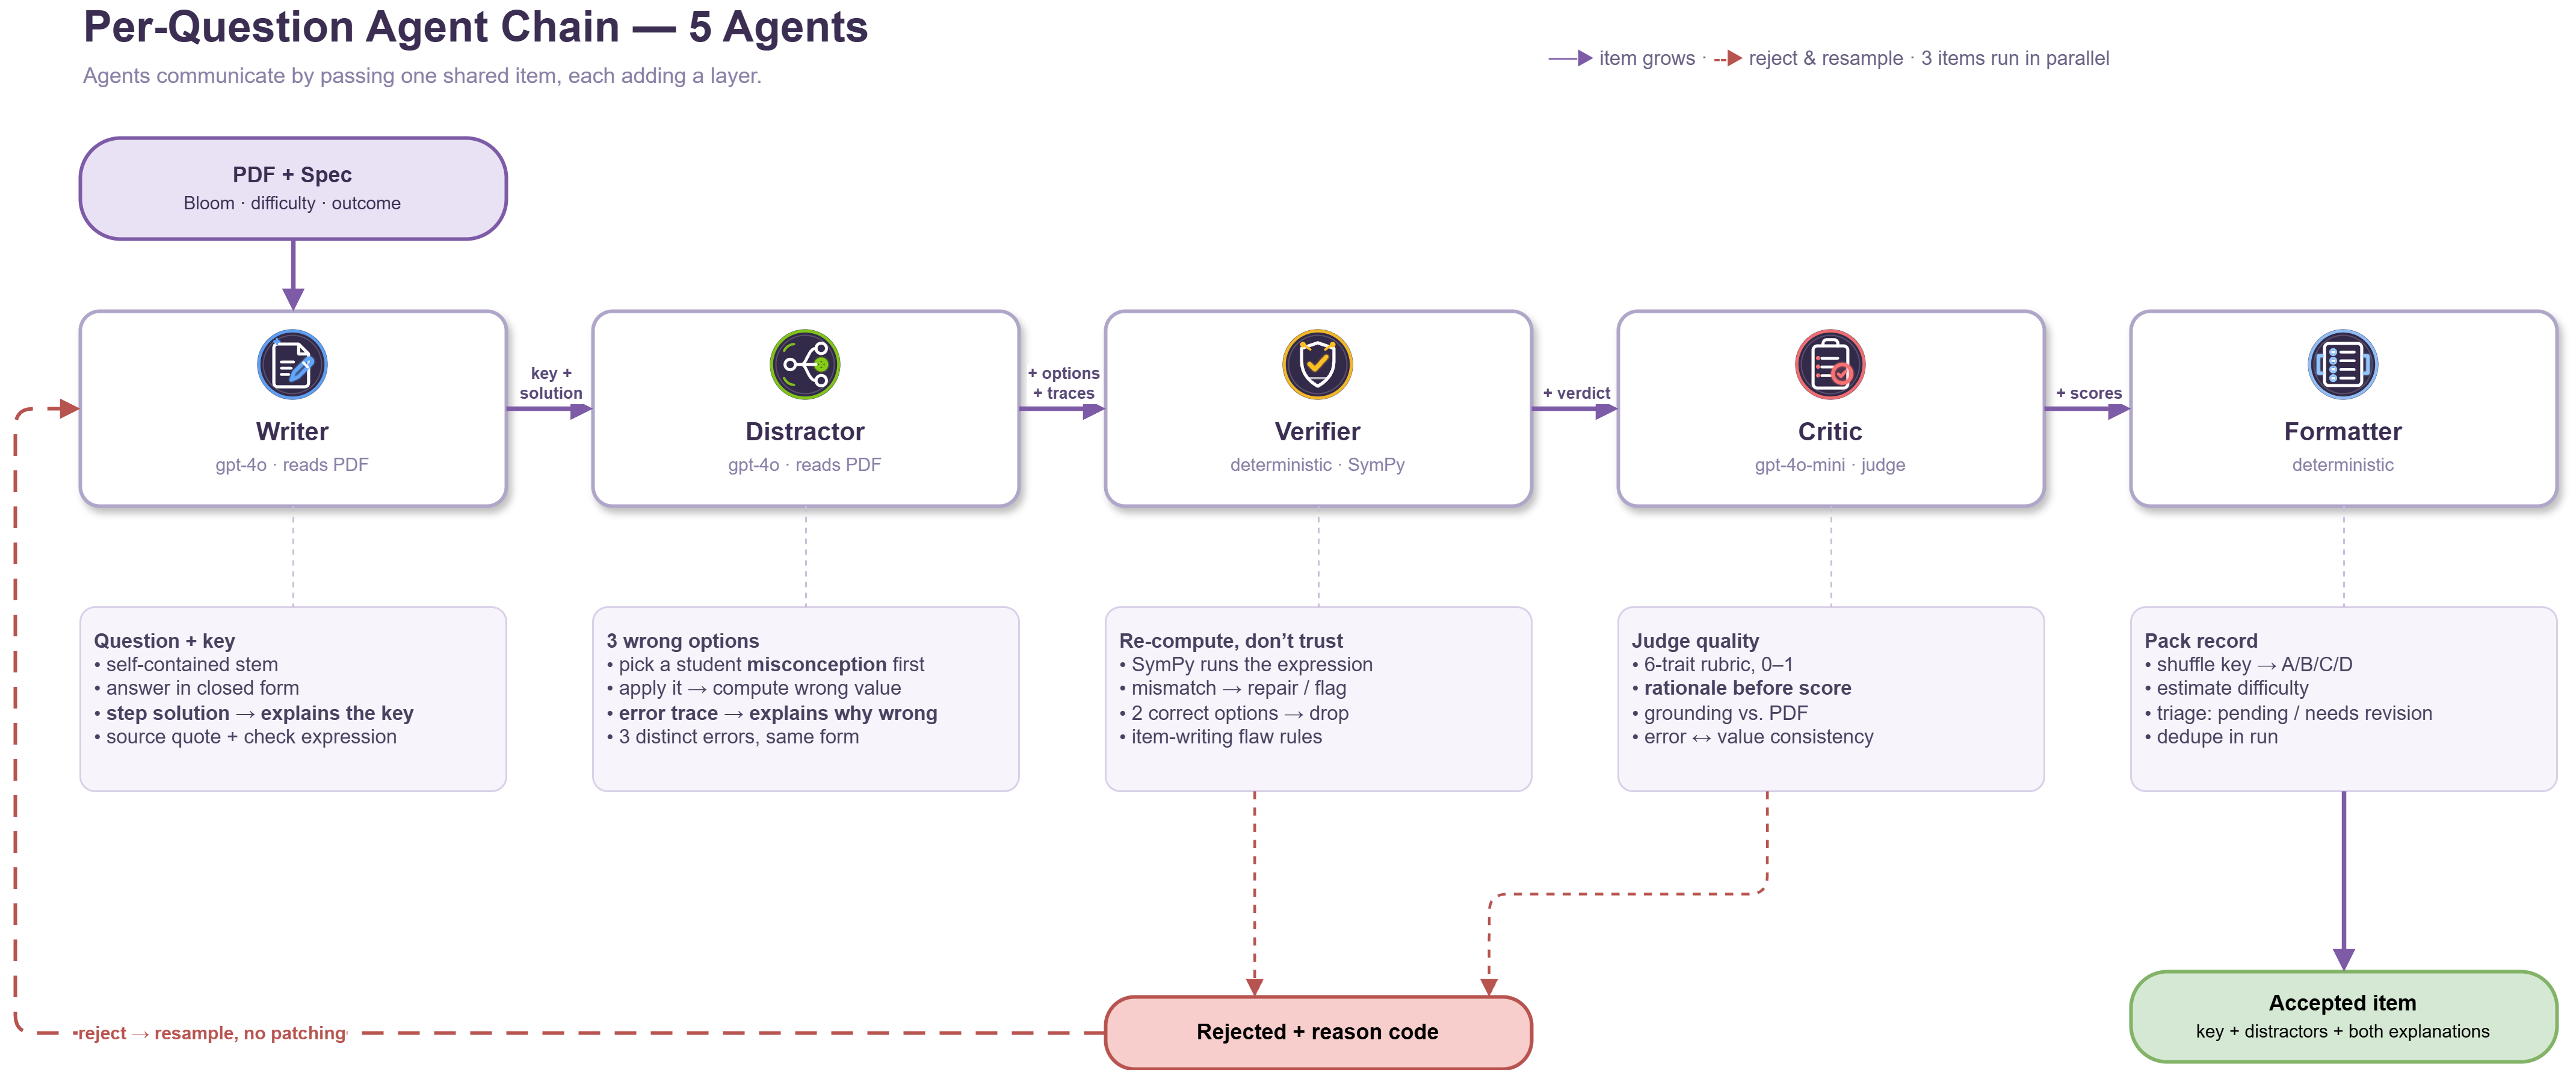
\includegraphics[width=0.95\textwidth]{../figs/pipeline-5-agent.png}
  \end{center}
  \vfill
  \note{
    Các tác tử giao tiếp một chiều bằng cách truyền một bản ghi dùng chung. Mỗi tác tử bồi thêm một lớp dữ liệu --- đó là các nhãn trên mũi tên liền.

    Verifier và Formatter là hai tác tử tất định.

    Đường nét đứt là các điểm loại bỏ. Mọi câu bị loại đều được ghi kèm mã lý do, và dẫn tới sinh lại một câu mới --- không vá câu cũ.
  }
\end{frame}

% =====================================================================
\begin{frame}{Luồng quyết định}
  \vfill
  \begin{center}
    \small
    \begin{tabular}{@{}l l@{}}
      \toprule
      \textbf{Cổng} & \textbf{Điều kiện đi tiếp} \\
      \midrule
      Writer      & Có ứng viên? \\
      Distractor  & Đủ ba nhiễu hợp lệ? \\
      \dt{Verifier}   & Không bị bác? Không đa đáp án? \\
      Critic      & Bám nguồn $\geq 0{,}4$? \ Duy nhất đáp án $\geq 0{,}5$? \ Nhất quán lỗi--giá trị $\geq 0{,}4$? \\
      \dt{Formatter}  & Định dạng hợp lệ? Không trùng câu đã nhận? \\
      \midrule
      \multicolumn{2}{@{}l@{}}{\dt{$\Rightarrow$ CHẤP NHẬN}} \\
      \bottomrule
    \end{tabular}
  \end{center}
  \vfill
  \punch{Bị loại ở cổng đầu tiên không đạt.\\[0.2em] $\Rightarrow$ sinh lại một câu mới, \textbf{không vá câu cũ}.}
  \vfill
  \srcnote{Mọi lần loại đều ghi kèm mã lý do và nhãn giai đoạn.}
  \note{
    Mỗi câu ứng viên đi qua một chuỗi cổng lọc nối tiếp, và bị loại tại cổng đầu tiên không đạt.

    Ba ngưỡng loại cứng ở tầng chấm: bám nguồn dưới 0,4; tính duy nhất đáp án dưới 0,5; nhất quán lỗi--giá trị dưới 0,4.

    Mọi lần loại đều được ghi kèm mã lý do và nhãn giai đoạn.
  }
\end{frame}

% =====================================================================
\section{Kỹ thuật}
\begin{frame}{Sinh bám tài liệu \emph{toàn văn}}
  \vfill
  \begin{columns}[T]
    \begin{column}{0.5\textwidth}
      \begin{block}{Không làm gì}
        \begin{itemize}
          \item Không trích xuất văn bản
          \item Không nhận dạng ký tự quang học
          \item Không chia đoạn nhỏ
        \end{itemize}
        \smallskip
        Tài liệu gốc đính kèm \alert{nguyên vẹn} cho cả ba tác tử dùng mô hình.
      \end{block}
    \end{column}
    \begin{column}{0.5\textwidth}
      \begin{block}{Vì sao}
        Giữ được bố cục, ký hiệu toán, bảng, hình --- những thứ bị \alert{phá huỷ} khi trích văn bản thô.
      \end{block}
      \begin{alertblock}{Cái giá}
        Token đầu vào cao. Giới hạn cứng độ dài tài liệu.
      \end{alertblock}
    \end{column}
  \end{columns}
  \vfill
  \punch{Bám nguồn \emph{nới lỏng}: được ra bài tập mới,\\[0.2em] miễn phương pháp nằm trong tài liệu.}
  \vfill
  \srcnote{Savaal \cite{22} cùng nhắm tài liệu dài, nhưng trích khái niệm rồi sinh theo khái niệm --- hệ thống giao toàn văn.}
  \note{
    Tài liệu được đóng gói một lần duy nhất và dùng chung cho toàn bộ các lời gọi mô hình về sau.

    Kiến trúc này khác hẳn hướng sinh câu hỏi dựa trên truy xuất đoạn văn: thay vì đưa cho mô hình một đoạn trích rồi hỏi, hệ thống đưa toàn bộ tài liệu ở dạng gốc và giao chỉ tiêu. Bố cục và ký hiệu toán học bị phá huỷ khi trích văn bản thô --- vấn đề kinh niên với học liệu Toán.

    Bám nguồn được thực thi qua hai cơ chế bổ trợ: Writer bắt buộc trích một đoạn nguyên văn 15--250 ký tự làm bằng chứng, và Critic nhận chính tài liệu đó để đối chiếu từng dữ kiện.

    Về chính sách nới lỏng: câu hỏi được phép là bài tập mới với số liệu, tên gọi, đơn vị hoặc tình huống đã thay đổi, miễn là công thức, định lý, phương pháp hoặc mô-típ bài mẫu nằm trong tài liệu. Đây là điều chỉnh bắt buộc --- nếu đòi hỏi mọi con số phải xuất hiện nguyên văn, hệ thống chỉ còn có thể chép lại bài tập có sẵn.
  }
\end{frame}

% =====================================================================
\begin{frame}{Lập lịch theo hạn ngạch \dg}
  \vfill
  \begin{columns}[T]
    \begin{column}{0.5\textwidth}
      \begin{block}{Mức Bloom}
        \alert{Round-robin có trọng số} theo phân bố khai báo.
      \end{block}
      \begin{block}{Chuẩn đầu ra}
        \alert{Least-covered-first} --- nhắm vào chuẩn đang phủ ít nhất.
        \smallskip
        Đếm cả câu \emph{đang sinh dở}.
      \end{block}
    \end{column}
    \begin{column}{0.5\textwidth}
      \begin{alertblock}{Vì sao đếm cả câu đang sinh dở}
        Khi song song, số câu \emph{đã xong} không phản ánh số câu \emph{đang nhắm tới}.
        \smallskip
        Một câu rớt giữa đợt $\Rightarrow$ chuẩn đầu ra của nó bỏ trống \textbf{vĩnh viễn}.
      \end{alertblock}
    \end{column}
  \end{columns}
  \vfill
  \punch{Giải phóng hạn ngạch khi thất bại\\[0.2em] $\Rightarrow$ phân bố tự cân bằng lại.}
  \vfill
  \srcnote{Thang phân loại nhận thức dùng trực tiếp từ \cite{8}. \quad \cite{23} cũng kết hợp mô hình ngôn ngữ với thang Bloom, nhưng không có cơ chế lập lịch hạn ngạch.}
  \note{
    Mỗi câu hỏi được ấn định sẵn mức Bloom, độ khó mục tiêu và một chuẩn đầu ra cụ thể trước khi bất kỳ lời gọi mô hình nào diễn ra.

    Vấn đề của song song: nếu chọn chuẩn đầu ra theo chỉ số tuần tự, một câu thất bại giữa đợt sẽ khiến chuẩn đầu ra của nó bị bỏ trống vĩnh viễn.

    Cơ chế đếm và giải phóng hạn ngạch khi thất bại làm cho phân bố tự cân bằng lại: nó trùng khớp với round-robin thuần khi mọi câu đều thành công, và tự bù chuẩn đầu ra bị hụt khi có câu rớt.

    Đây là một trong sáu điểm được đề xuất coi là đóng góp của hệ thống.
  }
\end{frame}

% =====================================================================
\begin{frame}{Tách vai và suy luận từng bước}
  \vfill
  \begin{columns}[T]
    \begin{column}{0.5\textwidth}
      \begin{block}{Sinh hai giai đoạn}
        Writer chỉ sinh \textbf{lõi} câu hỏi --- \alert{bị cấm sinh nhiễu}.
        \smallskip
        Nhiễu giao hẳn cho tác tử kế tiếp.
        \smallskip
        \textbf{Giá:} hai lời gọi thay vì một.
      \end{block}
      \srcnote{Nguyên lý tách vai từ \cite{4}, có điều chỉnh --- không dùng cơ chế chọn mẫu ví dụ.}
    \end{column}
    \begin{column}{0.5\textwidth}
      \begin{block}{Suy luận từng bước}
        Các bước đánh số, \alert{số bước tối thiểu tăng theo Bloom} (2/3/4/5).
        \smallskip
        Cấm in suy luận nháp.
      \end{block}
      \begin{alertblock}{Khác chain-of-thought gốc}
        Ở \cite{5}: chuỗi suy luận là \emph{phương tiện}, bỏ đi sau khi lấy đáp án.
        \smallskip
        Ở đây: nó là \alert{sản phẩm cuối} --- lời giải cho học sinh.
      \end{alertblock}
    \end{column}
  \end{columns}
  \vfill
  \note{
    Tách vai: mỗi lời gọi mô hình tập trung vào một việc. Writer sinh đề bài, đáp án đúng, lời giải, trích dẫn nguồn, biểu thức kiểm chứng. Tác tử sinh nhiễu đã có sẵn đáp án đúng và lời giải làm đầu vào.

    Đánh đổi: tăng số lời gọi mô hình cho mỗi câu --- chi phí được chấp nhận có ý thức.

    Chain-of-Exemplar đề xuất tách và cấu trúc hoá quá trình sinh phương án nhiễu. Hệ thống áp dụng nguyên lý tách vai nhưng không dùng cơ chế chọn mẫu ví dụ của bài báo.

    Về suy luận từng bước: vì chuỗi suy luận vừa là phương tiện vừa là sản phẩm cuối, nó bị ràng buộc về hình thức trình bày và độ dài tối thiểu --- điều không có trong bài báo gốc.
  }
\end{frame}

% =====================================================================
\begin{frame}{Sinh nhiễu \emph{error-first} \dg}
  \vspace{1em}
  \begin{center}
  \begin{tikzpicture}[
      node distance=0.9cm,
      st/.style = {draw=cAccent, fill=cAccent!8, rounded corners=3pt, minimum height=2.8em, text width=3.4cm, align=center, font=\small},
      ar/.style = {-{Latex[length=2mm]}, draw=cAccent, thick} ]
    \node[st] (a) {Chọn \emph{trước} một lỗi\\điển hình của học sinh};
    \node[st, right=of a] (b) {\emph{Áp lỗi} vào bài toán\\để \emph{tính ra} giá trị sai};
    \node[st, right=of b] (c) {Ghi giá trị đó\\thành phương án};
    \draw[ar] (a) -- (b);  \draw[ar] (b) -- (c);
  \end{tikzpicture}
  \end{center}
  \vfill
  \punch{Mỗi phương án kèm mô tả chuỗi bước làm sai ---\\[0.2em] làm đúng chuỗi đó phải ra \emph{đúng} giá trị ấy.}
  \vfill
  \begin{center}
    \small Tính hợp lý của nhiễu --- vốn \textbf{chủ quan} --- thành \alert{mệnh đề kiểm chứng được}.
  \end{center}
  \vfill
  \srcnote{\cite{9}, \cite{10}, \cite{29} cùng đặt quan niệm sai lầm làm trung tâm; hệ thống dùng prompting có ràng buộc, \textbf{không huấn luyện}.}
  \note{
    Quy trình đảo ngược thứ tự thông thường: chọn lỗi trước, rồi mới tính ra giá trị sai --- thay vì bịa một con số trông giống đáp án.

    Hệ thống duy trì sẵn một danh mục quan niệm sai lầm phổ biến theo chủ đề. Mỗi bài toán được ghép với một nhóm nhỏ các lỗi khớp nội dung nhất. Việc chọn dùng hạt giống ngẫu nhiên cố định theo nội dung bài, nên cùng một bài luôn nhận cùng danh sách --- bảo đảm tái lập khi gỡ lỗi hoặc đo đạc.

    Ràng buộc bổ sung: ba phương án phải dùng ba lỗi khác nhau, cùng dạng và cùng đơn vị với đáp án đúng.

    Câu chốt là đóng góp quan trọng nhất của phần này: nó biến một phẩm chất chủ quan thành mệnh đề kiểm chứng được, và chính mệnh đề này được đưa cho Critic chấm.
  }
\end{frame}

% =====================================================================
\begin{frame}{Kiểm chứng bằng chương trình}
  \punch{Tách năng lực \emph{giải toán}\\[0.2em] khỏi năng lực \emph{tự chấm}.}
  \vfill
  \begin{columns}[T]
    \begin{column}{0.5\textwidth}
      \begin{block}{Cách làm}
        Writer viết kèm một \textbf{biểu thức kiểm chứng máy đọc được} --- hơn 20 loại.
        \smallskip
        Biểu thức được \alert{chạy thật} bằng thư viện tính toán ký hiệu \cite{11}.
      \end{block}
    \end{column}
    \begin{column}{0.5\textwidth}
      \begin{alertblock}{Khác PAL / PoT \cite{6}, \cite{7}}
        Ở đó: chương trình \emph{giải} bài, kết quả \emph{chính là} đáp án --- \textbf{một nguồn}.
        \smallskip
        Ở đây: chương trình \emph{kiểm chứng} lời giải --- \alert{hai nguồn độc lập}.
      \end{alertblock}
    \end{column}
  \end{columns}
  \vfill
  \punch{Hai nguồn $\Rightarrow$ phát hiện được bất đồng.}
  \vfill
  \note{
    Hơn hai mươi loại biểu thức kiểm chứng: giải phương trình, đạo hàm, tích phân, giới hạn, định thức, giá trị riêng, tổ hợp, xác suất, số học mô-đun, tương đương logic, tính chất đồ thị...

    Cách chạy: thư viện tính toán ký hiệu, kết hợp đối chiếu số học tại nhiều điểm. Đáp án do đó được máy tính lại, không phải do mô hình tự nhận là đúng.

    Với các câu hỏi khái niệm không thể kiểm bằng máy, hệ thống cho phép khai báo loại "không kiểm chứng" thay vì ép một biểu thức khiên cưỡng.

    Điểm mấu chốt so với PAL và Program-of-Thought: ở đó chỉ có một nguồn kết quả duy nhất nên không có gì để đối chiếu. Ở đây mô hình vẫn tự giải bằng ngôn ngữ tự nhiên, còn chương trình là nguồn thứ hai độc lập.

    Đây là chốt chặn đặc thù môn Toán mà các pipeline AQG thuần mô hình ngôn ngữ không có, và là nền tảng cho ba kỹ thuật ở slide sau.
  }
\end{frame}

% =====================================================================
\begin{frame}{Ba kỹ thuật dẫn xuất --- cả ba đều là đóng góp \dg}
  \vfill
  \begin{columns}[T]
    \begin{column}{0.33\textwidth}
      \begin{block}{Loại trừ đa đáp án}
        Chạy bộ kiểm chứng trên \emph{cả ba nhiễu}.
        \smallskip
        Một nhiễu cũng đúng $\Rightarrow$ \alert{loại cả câu}.
        \smallskip
        \textbf{Bằng chứng máy} cho việc đề có nhiều đáp án.
      \end{block}
    \end{column}
    \begin{column}{0.33\textwidth}
      \begin{block}{Tự sửa đáp án}
        Đáp án lệch, nhưng một nhiễu lại khớp?
        \smallskip
        $\Rightarrow$ Hoán đổi hai bên, viết lại lời giải.
        \smallskip
        Cứu câu \alert{đúng nhưng dán nhầm nhãn}.
      \end{block}
    \end{column}
    \begin{column}{0.33\textwidth}
      \begin{alertblock}{``Không khớp $\neq$ sai''}
        Chỉ \textbf{1/12} ca lệch là sai thật --- phần lớn do \emph{biểu thức viết sai đề}.
        \smallskip
        {\scriptsize\color{cMuted}(ghi nhận vận hành)}
        \smallskip
        $\Rightarrow$ Giữ câu, \alert{ép duyệt tay}.
      \end{alertblock}
    \end{column}
  \end{columns}
  \vfill
  \punch{Nghiêng về recall --- vì đã có tầng con người phía sau.}
  \vfill
  \note{
    Loại trừ đa đáp án: kỹ thuật này chỉ khả thi nhờ ràng buộc phương án nhiễu phải cùng dạng với đáp án đúng.

    Tự sửa đáp án: hệ thống hoán đổi hai bên, viết lại các tham chiếu số trong lời giải cho nhất quán, và ghi chú lại thao tác. Nó cứu được lớp câu hỏi đúng về bản chất nhưng dán nhầm nhãn --- một lỗi rất phổ biến và rất phí nếu vứt cả câu.

    Chính sách "không khớp không có nghĩa là sai": cơ sở là một quan sát vận hành --- phần lớn ca lệch xuất phát từ việc biểu thức kiểm chứng được viết không đúng đề, chứ không phải mô hình giải sai. Theo ghi nhận trong tài liệu hệ thống, chỉ khoảng 1 trên 12 ca lệch là sai thật.

    Lưu ý con số 1/12 là ghi nhận vận hành, không phải kết quả thí nghiệm có đối chứng.

    Đây là một đánh đổi có ý thức giữa precision và recall, nghiêng về recall.
  }
\end{frame}

% =====================================================================
\begin{frame}{Kiểm soát độ khó \emph{hai trục} \dg}
  \punch{Chỉ ràng buộc Bloom $\Rightarrow$ mô hình đúng \emph{hình thức}\\[0.2em] nhưng vẫn chọn số liệu dễ nhất.}
  \vfill
  \begin{columns}[T]
    \begin{column}{0.5\textwidth}
      \begin{block}{Trục 1 --- Số bước suy luận}
        Ràng buộc bằng mức Bloom.
        \smallskip
        Vận dụng cao: bắt buộc phối hợp $\geq$ 2 kỹ thuật.
      \end{block}
    \end{column}
    \begin{column}{0.5\textwidth}
      \begin{block}{Trục 2 --- Độ nặng phép tính}
        Điều kiện \textbf{leo thang} theo độ khó.
        \smallskip
        \alert{Cấm bộ số kinh điển} của dạng bài.
      \end{block}
    \end{column}
  \end{columns}
  \vfill
  \begin{alertblock}{Cơ sở nghiên cứu}
    \centering \textbf{Không thể xác nhận từ mã nguồn hoặc tài liệu được cung cấp.}\\
    Kỹ thuật này xuất phát từ quan sát vận hành nêu trên.
  \end{alertblock}
  \vfill
  \note{
    Trục số bước suy luận: từ mức Thông hiểu trở lên cấm hỏi định nghĩa chép lại; mức Vận dụng cao bắt buộc phối hợp từ hai kỹ thuật trở lên.

    Trục độ nặng phép tính: cấm dùng bộ số kinh điển của dạng bài; mức giữa buộc phải có dữ kiện mà người học tự biến đổi mới ra được; mức cao nhất buộc ra bài chứa tham số, bài ngược, hoặc phối hợp kỹ thuật.

    Về cơ sở: đây là một trong ba chỗ trong báo cáo phải ghi rõ là không xác nhận được từ tài liệu. Kỹ thuật xuất phát từ quan sát vận hành: khi chỉ ràng buộc mức Bloom, mô hình đáp ứng đúng hình thức của mức nhận thức nhưng chọn số liệu dễ nhất có thể, khiến độ khó thực tế không đổi giữa các mức.
  }
\end{frame}

% =====================================================================
\section{Kiểm soát chất lượng}
\begin{frame}{Đánh giá dựa trên rubric}
  \vfill
  \begin{block}{Sáu tiêu chí, thang $0$--$1$}
    \centering
    rõ ràng $\cdot$ chiều sâu tư duy $\cdot$ khớp Bloom $\cdot$ hợp lý của nhiễu $\cdot$ \alert{duy nhất đáp án} $\cdot$ \alert{nhất quán lỗi--giá trị}
  \end{block}
  \vfill
  \begin{columns}[T]
    \begin{column}{0.5\textwidth}
      \begin{block}{Model bất đối xứng}
        Model chấm \alert{nhẹ hơn} model sinh.
        \smallskip
        \emph{Chấm dễ hơn sinh.} \quad \cite{13}
      \end{block}
    \end{column}
    \begin{column}{0.5\textwidth}
      \begin{block}{Nhận định trước, điểm sau}
        Viết nhận định \emph{rồi mới} cho điểm --- từng tiêu chí.
        \smallskip
        Nguyên lý từ \cite{14}, chuyển miền: bài luận $\rightarrow$ MCQ.
      \end{block}
    \end{column}
  \end{columns}
  \vfill
  \punch{``Nhất quán lỗi--giá trị'' bắt lớp lỗi\\[0.2em] \emph{giải thích một đằng, con số một nẻo}.}
  \vfill
  \note{
    Điểm chất lượng tổng là trung bình của sáu tiêu chí. Ba tiêu chí có ngưỡng loại cứng riêng: bám nguồn dưới 0,4; duy nhất đáp án dưới 0,5; nhất quán lỗi--giá trị dưới 0,4.

    Model bất đối xứng: lập luận là chấm là bài toán dễ hơn sinh, dùng mô hình lớn cho việc này là lãng phí. MT-Bench thiết lập tính khả dụng của mô hình ngôn ngữ trong vai trò giám khảo; việc chọn model chấm nhẹ hơn là một điều chỉnh về chi phí, không phải kết luận của bài báo.

    Nhận định trước, điểm sau: chống lại thói cho điểm bừa rồi bịa lý do biện minh. Bản thân nhận định được lưu lại làm bằng chứng hiển thị cho người duyệt. RMTS đề xuất nguyên lý này cho chấm bài luận; hệ thống chuyển miền sang chấm câu hỏi trắc nghiệm với bộ tiêu chí khác hoàn toàn.

    Tiêu chí nhất quán lỗi--giá trị kiểm hai mệnh đề: thực hiện đúng chuỗi lỗi mà tác tử sinh nhiễu mô tả có ra đúng giá trị phương án đó không; và lời giải có nhất quán với đáp án không. Nó bắt lớp lỗi mà kiểm chứng ký hiệu không thấy được, vì kiểm chứng chỉ soi đáp án đúng.
  }
\end{frame}

% =====================================================================
\begin{frame}{Hai tầng bảo vệ ở khâu chấm}
  \vfill
  \begin{columns}[T]
    \begin{column}{0.5\textwidth}
      \begin{alertblock}{Fail-open}
        Tác tử chấm lỗi $\Rightarrow$ câu \textbf{không bị chặn}: điền điểm trung tính, để người duyệt quyết.
        \smallskip
        Đầu ra cắt cụt $\Rightarrow$ \textbf{vớt điểm từng phần}.
      \end{alertblock}
      \punch{Lỗi hạ tầng ở khâu chấm\\ không được giết oan cả lượt sinh.}
    \end{column}
    \begin{column}{0.5\textwidth}
      \begin{block}{Soát lỗi soạn đề --- tất định}
        \begin{itemize}
          \item Nhiễu trùng nhau
          \item Từ tuyệt đối ``luôn luôn''
          \item Thang số không cân đối
          \item Định dạng không đồng nhất
          \item Mỗi nhiễu một lỗi khác nhau
        \end{itemize}
      \end{block}
      \srcnote{Bộ hướng dẫn từ \cite{12}; hệ thống chỉ triển khai tập con \emph{diễn đạt được thành vị từ máy kiểm}.}
    \end{column}
  \end{columns}
  \vfill
  \note{
    Fail-open: nếu tác tử chấm gặp sự cố hoặc kết quả không phân tích được, hệ thống điền điểm trung tính và để tầng đóng gói cùng người duyệt quyết định. Bổ sung cho cơ chế này là bước vớt điểm từng phần khi đầu ra bị cắt cụt giữa chừng --- các tiêu chí đã chấm xong vẫn giữ được điểm thật thay vì toàn bộ rơi về trung tính.

    Lưu ý: fail-open có mặt trái, sẽ nói ở phần hạn chế --- nó làm loãng tín hiệu, khiến điểm của một số câu phản ánh sự cố hạ tầng chứ không phải chất lượng thật.

    Soát lỗi soạn đề: bộ quy tắc rút từ lĩnh vực đo lường giáo dục, hoàn toàn tất định, không gọi mô hình. Từ tuyệt đối kiểu "luôn luôn"/"không bao giờ" trong nhiễu thì học sinh học được mẹo loại trừ. Thang số không cân đối nghĩa là phương án lệch quá xa về độ lớn so với trung vị thì dễ đoán.

    Haladyna và cộng sự tổng hợp bộ hướng dẫn soạn MCQ từ nghiên cứu đo lường giáo dục. Hệ thống chỉ chuyển tập con các hướng dẫn có thể diễn đạt thành vị từ máy kiểm được thành quy tắc tự động; phần còn lại mang tính định tính.
  }
\end{frame}

% =====================================================================
\begin{frame}{Sinh lại, không vá}
  \vfill
  \punch{Câu bị loại được \textbf{thay bằng một câu sinh mới} ---\\[0.2em] không phải sửa cục bộ.}
  \vfill
  \begin{columns}[T]
    \begin{column}{0.5\textwidth}
      \begin{block}{1. Chi phí}
        Một vòng sửa cần một lời gọi mô hình, cộng chi phí kiểm định lại toàn chuỗi.
        \smallskip
        $\Rightarrow$ \alert{Không rẻ hơn sinh mới bao nhiêu.}
      \end{block}
    \end{column}
    \begin{column}{0.5\textwidth}
      \begin{alertblock}{2. Trạng thái sạch}
        Vá cục bộ làm \emph{bất nhất} các ràng buộc chéo:
        \smallskip
        \centerline{\small đáp án $\leftrightarrow$ lời giải $\leftrightarrow$ biểu thức $\leftrightarrow$ mô tả lỗi}
        \smallskip
        $\Rightarrow$ Tự tạo ra \alert{đúng lớp lỗi} mà tiêu chí nhất quán lỗi--giá trị dựng ra để bắt.
      \end{alertblock}
    \end{column}
  \end{columns}
  \vfill
  \srcnote{\cite{1}, \cite{2} cùng theo hướng sinh dư rồi lọc, thay vì tin một lượt sinh duy nhất. \quad \cite{19} đi hướng ngược lại: tự phê bình, tự sửa, so sánh lặp.}
  \note{
    Câu bị loại ở bất kỳ cổng nào sẽ bị thay bằng một câu sinh mới. Hệ thống không có tác tử Refiner --- đây là lựa chọn có chủ ý, dựa trên hai lập luận.

    Lập luận chi phí: một vòng sửa cần ít nhất một lời gọi mô hình, cộng thêm chi phí kiểm định lại toàn chuỗi.

    Lập luận trạng thái --- đây mới là lập luận chính: một câu đã sửa mang theo lịch sử của phiên bản hỏng. Các ràng buộc chéo giữa đáp án, lời giải, biểu thức kiểm chứng và mô tả lỗi rất dễ trở nên bất nhất sau khi vá cục bộ. Mà đó chính là lớp bất nhất mà tiêu chí nhất quán lỗi--giá trị được dựng ra để bắt. Vá cục bộ tức là tự tạo ra đúng thứ mình đang cố phát hiện.

    NẾU BỊ HỎI "sao không cho agent sửa lại cho đỡ tốn": trả lời bằng đúng hai lập luận trên. Nếu bị truy tiếp "đã đo chưa" --- trả lời thẳng: đây là lập luận thiết kế, chưa so sánh thực nghiệm với hướng sửa lặp của MCQG-SRefine.

    NẾU BỊ HỎI "sao các tác tử không tranh luận với nhau": các tác tử giao tiếp một chiều theo chuỗi, không thương lượng. Có bài báo cho thấy tranh luận đa tác tử có các chế độ thất bại đáng kể và không phải lúc nào cũng cải thiện chất lượng suy luận.
  }
\end{frame}

% =====================================================================
\begin{frame}{Phân luồng và nhật ký loại bỏ \dg}
  \vfill
  \begin{columns}[T]
    \begin{column}{0.5\textwidth}
      \begin{block}{Phân luồng cho người duyệt}
        \begin{itemize}
          \item Duy nhất đáp án thấp / lệch Bloom $\Rightarrow$ \textbf{ép điểm xuống} + cần sửa
          \item Sát ngưỡng $\Rightarrow$ cần sửa
          \item Kiểm chứng lệch $\Rightarrow$ cần sửa, \alert{không trừ điểm}
          \item Còn lại $\Rightarrow$ chờ duyệt
        \end{itemize}
      \end{block}
    \end{column}
    \begin{column}{0.5\textwidth}
      \begin{block}{Nhật ký loại bỏ có mã lý do}
        Mọi câu bị loại: \textbf{mã lý do} + \textbf{nhãn giai đoạn}, hiển thị cho người dùng.
        \smallskip
        Câu bị loại thành \alert{dữ liệu chẩn đoán}.
      \end{block}
      \punch{``Hỏng ở khâu nào?''\\ thay vì ``tỉ lệ đạt thấp''.}
    \end{column}
  \end{columns}
  \vfill
  \begin{center}
    \small Tách \textbf{hạ điểm} khỏi \textbf{buộc duyệt tay} $\Rightarrow$ biểu đạt được \emph{sự không chắc chắn} mà không làm sai lệch \emph{thứ hạng}.
  \end{center}
  \vfill
  \note{
    Mọi tín hiệu nghi ngờ tích luỹ dọc pipeline được quy về một trong hai trạng thái, kèm danh sách lý do: cần sửa, hoặc chờ duyệt.

    Chi tiết quan trọng nhất ở đây: kiểm chứng toán không khớp thì luôn chuyển vào diện cần sửa, nhưng không trừ điểm. Theo đúng chính sách "không khớp không phải là sai" --- một câu đúng mà biểu thức kiểm chứng viết lệch vẫn phải được xếp hạng công bằng so với các câu khác.

    Sự tách bạch giữa hạ điểm và buộc duyệt tay cho phép hệ thống biểu đạt sự không chắc chắn mà không làm sai lệch thứ hạng chất lượng. Đây là một trong sáu đóng góp được đề xuất.

    Nhật ký loại bỏ: mọi điểm loại --- không sinh được, thiếu nhiễu, bị kiểm chứng bác, chấm rớt, đóng gói lỗi, trùng lặp, lỗi hệ thống. Giữ tối đa một số lượng bản ghi nhất định mỗi lượt để tránh phình dữ liệu khi mô hình lỗi hàng loạt.

    Đây là điều kiện cần để đo đạc và cải tiến từng cổng lọc một cách độc lập.

    Còn một chi tiết nữa ở tầng đóng gói: đáp án đúng được xáo ngẫu nhiên vào bốn vị trí, và các tham chiếu tới nhãn phương án trong lời giải được viết lại cho khớp. Bài báo [15] chứng minh mô hình ngôn ngữ chịu thiên lệch vị trí --- họ khử thiên lệch ở phía chọn, hệ thống trộn ở phía sinh.
  }
\end{frame}

% =====================================================================
\section{Phản hồi}
\begin{frame}{Vòng lặp con người}
  \vfill
  \begin{columns}[T]
    \begin{column}{0.5\textwidth}
      \begin{block}{Cùng một phiên --- không tải lại tài liệu}
        \begin{itemize}
          \item Duyệt từng câu
          \item Sinh lại câu bị chê
          \item Sinh thêm
          \item Luyện tập thử
          \item Xuất bản
        \end{itemize}
      \end{block}
    \end{column}
    \begin{column}{0.5\textwidth}
      \begin{block}{Ba mức phản hồi}
        \begin{itemize}
          \item Đánh giá nhị phân
          \item \alert{Thẻ lý do có cấu trúc}
          \item Bình luận tự do
        \end{itemize}
      \end{block}
      \begin{alertblock}{Mỗi thẻ $\rightarrow$ một chỉ thị hành động}
        ``Quá dễ'' $\rightarrow$ \emph{tăng số bước biến đổi, cấm hỏi chép lại định nghĩa}.
      \end{alertblock}
    \end{column}
  \end{columns}
  \vfill
  \punch{Tổng hợp thẻ là \dt{tất định} --- không tốn chi phí suy luận.}
  \vfill
  \note{
    Toàn bộ các thao tác ở cột trái diễn ra trên cùng một phiên làm việc. Sinh lại chỉ thay các câu bị đánh giá kém, các câu còn lại giữ nguyên.

    Bộ thẻ lý do phía tiêu cực: quá dễ, quá khó, đề mơ hồ, nghi sai đáp án, nhiễu kém, lệch tài liệu, trùng dạng. Phía tích cực: độ khó phù hợp, ngữ cảnh hay, giải thích rõ, nhiễu tốt.

    Việc dùng thẻ có cấu trúc thay vì chỉ bình luận tự do là một quyết định phương pháp: nó khiến phần lớn quá trình tổng hợp phản hồi trở nên tất định và không tốn chi phí suy luận, đồng thời cho ra chỉ thị chính xác hơn so với việc để mô hình tự diễn giải văn bản tự do. Chỉ phần cô đọng bình luận tự do mới cần gọi mô hình, và đây là bước best-effort --- lỗi thì liệt kê thô.

    Có hai cơ chế độc lập: hồ sơ sở thích điều hướng phong cách, còn danh sách tránh lặp (đề bài của mọi câu cũ, kể cả câu bị chê) ngăn trùng nội dung.
  }
\end{frame}

% =====================================================================
\begin{frame}{Học sở thích \emph{trong ngữ cảnh}}
  \vfill
  \begin{columns}[T]
    \begin{column}{0.5\textwidth}
      \begin{block}{\cite{3} --- RLHF}
        Huấn luyện mô hình phần thưởng $\rightarrow$ tinh chỉnh chính sách bằng học tăng cường.
      \end{block}
    \end{column}
    \begin{column}{0.5\textwidth}
      \begin{alertblock}{Hệ thống --- giữ ý tưởng, bỏ phần huấn luyện}
        Giữ \textbf{tín hiệu} và \textbf{mục tiêu}.
        \smallskip
        \alert{Bỏ hoàn toàn phần huấn luyện} --- điều hướng qua ngữ cảnh.
      \end{alertblock}
    \end{column}
  \end{columns}
  \vfill
  \begin{block}{Đánh đổi}
    \centering
    Hiệu lực tức thì, chi phí huấn luyện bằng không\\
    $\longleftrightarrow$\\
    Sở thích không nội tại hoá vào trọng số; trả phí token lặp lại mọi lượt
  \end{block}
  \vfill
  \srcnote{Ở \cite{27}, \cite{29} phản hồi chuyên gia dùng để \emph{đánh giá} hệ thống; ở đây nó tác động \textbf{thời gian thực} lên câu sinh kế tiếp.}
  \note{
    Đây là một điều chỉnh đáng kể so với bài báo gốc, không phải áp dụng trực tiếp.

    Cách làm: phản hồi của người dùng cho từng câu được tổng hợp thành một khối chỉ dẫn dạng văn bản, rồi tiêm thẳng vào ngữ cảnh của Writer và Distractor ở các lượt sau.

    Hồ sơ sở thích được lưu bền theo phiên làm việc, nên mọi lượt sinh sau --- kể cả sinh thêm ở một thời điểm khác --- vẫn tôn trọng phản hồi đã cho. Đây là điểm phân biệt với việc chỉ áp phản hồi cho đúng một lượt sinh lại.

    Về đối chiếu: ở các bài báo về phản hồi chuyên gia, phản hồi chủ yếu được dùng để đánh giá hệ thống hoặc định nghĩa chiến lược trước khi chạy. Ở đây nó được đưa trở lại vòng sinh trong thời gian thực.
  }
\end{frame}

% =====================================================================
\section{Ngân hàng}
\begin{frame}{Khử trùng lặp ba tầng}
  \punch{Xếp theo \emph{chi phí tăng dần} --- bắt được ở tầng rẻ thì không chạy tầng đắt.}
  \vfill
  \begin{columns}[T]
    \begin{column}{0.31\textwidth}
      \begin{block}{1 --- Nguyên văn}
        So khớp sau chuẩn hoá.
        \smallskip
        Chi phí $\approx 0$.
      \end{block}
    \end{column}
    \begin{column}{0.31\textwidth}
      \begin{block}{2 --- Hình thái}
        Tương tự chuỗi, ngưỡng $0{,}85$.
        \smallskip
        Bắt khác vài từ, dấu câu.
      \end{block}
    \end{column}
    \begin{column}{0.38\textwidth}
      \begin{alertblock}{3 --- Ngữ nghĩa}
        Nhúng + cosine, ngưỡng $0{,}82$. \quad \cite{16}
        \smallskip
        Tầng \textbf{duy nhất} bắt được: \alert{cùng bài toán, diễn đạt khác hoặc thay số}.
      \end{alertblock}
    \end{column}
  \end{columns}
  \vfill
  \begin{center}
    \small Không có nhúng $\Rightarrow$ so từng cặp bằng mô hình ngôn ngữ: \textbf{bậc hai} theo kích thước kho.\\
    Ghi nhận vận hành: \textbf{$\approx$42 giây} $\rightarrow$ \textbf{$\approx$4 giây}.
  \end{center}
  \vfill
  \note{
    Ba tầng xếp theo thứ tự chi phí tăng dần --- một câu đã bị bắt ở tầng rẻ thì không cần chạy tầng đắt.

    Tầng 3 là tầng duy nhất bắt được lớp trùng nguy hiểm nhất: cùng một bài toán được diễn đạt khác đi hoặc thay số liệu. Câu cũ trong ngân hàng chưa có vector nhúng được bổ sung tự động ngay trong lần so đầu tiên, nên hệ thống không cần một bước di trú dữ liệu riêng khi bật tính năng này.

    Việc dùng một nhà cung cấp nhúng tách rời khỏi nhà cung cấp mô hình chat là một quyết định kỹ thuật thuần tuý --- không phải mọi cổng truy cập mô hình chat đều mở endpoint nhúng.

    Con số 42 giây xuống 4 giây minh hoạ vì sao khử trùng lặp ngữ nghĩa bằng nhúng là lựa chọn khả mở duy nhất khi ngân hàng lớn dần. Lưu ý đây là ghi nhận vận hành, không phải kết quả thí nghiệm.
  }
\end{frame}

% =====================================================================
\begin{frame}{Khi phát hiện trùng: ai quyết?}
  \vfill
  \punch{Hệ thống \emph{không} tự động loại.}
  \vfill
  \begin{center}
    \begin{tikzpicture}[
        opt/.style = {draw=cPrimary, fill=cBg, rounded corners=3pt, minimum height=3em, text width=3.2cm, align=center, font=\small} ]
      \node[opt, fill=cDet!10, draw=cDet] (a) {\textbf{Bỏ qua}\\{\footnotesize(mặc định)}};
      \node[opt, right=0.8cm of a] (b) {\textbf{Thay thế}\\{\footnotesize câu cũ}};
      \node[opt, right=0.8cm of b] (c) {\textbf{Vẫn thêm}};
    \end{tikzpicture}
  \end{center}
  \vfill
  \begin{center}
    \small Hai câu tương tự vẫn có thể \emph{đều hữu ích} --- ví dụ hai phiên bản của cùng một đề.\\
    Chỉ người dùng mới biết ý định sử dụng.
  \end{center}
  \vfill
  \punch{Khi không chắc: chuyển việc cho con người \emph{kèm lý do} --- thay vì đoán.}
  \vfill
  \note{
    Hệ thống trình bày cặp câu trùng kèm loại trùng và điểm số cho người dùng, với ba lựa chọn.

    Câu chốt cuối là nguyên tắc chung xuyên suốt hệ thống --- sẽ quay lại ở phần kết luận. Cùng nguyên tắc này giải thích chính sách "không khớp không phải là sai", cơ chế fail-open ở tầng chấm, và cơ chế tự sửa đáp án.
  }
\end{frame}

% =====================================================================
\section{Đối chiếu}
\begin{frame}{Đối chiếu: dùng trực tiếp và có điều chỉnh}
  \vspace{0.1em}
  \begin{center}
  \scriptsize
  \setlength{\tabcolsep}{4pt}
  \renewcommand{\arraystretch}{0.95}
  \begin{tabular}{@{}l c l@{}}
    \toprule
    \textbf{Kỹ thuật} & \textbf{Bài báo} & \textbf{Hệ thống bổ sung gì} \\
    \midrule
    Thang Bloom                  & \cite{8}  & \dt{Dùng trực tiếp} + gắn độ khó mục tiêu mỗi mức \\
    Kiểm chứng ký hiệu           & \cite{11} & \dt{Dùng trực tiếp} + để kiểm chứng, không phải giải toán \\
    Nhúng ngữ nghĩa              & \cite{16} & \dt{Dùng trực tiếp} + đặt sau hai tầng lọc rẻ hơn \\
    \midrule
    Kiểm chứng bằng chương trình & \cite{6}, \cite{7} & \alert{Kiểm chứng lời giải chứ không thay thế} $\Rightarrow$ hai nguồn \\
    Suy luận từng bước           & \cite{5}  & \alert{Chuỗi suy luận thành sản phẩm cuối} + ràng buộc số bước \\
    Tách lõi khỏi nhiễu          & \cite{4}  & Giữ nguyên lý tách vai, bỏ cơ chế chọn mẫu ví dụ \\
    Học sở thích người dùng      & \cite{3}  & \alert{Bỏ hoàn toàn phần huấn luyện} $\Rightarrow$ hiệu lực tức thì \\
    Nhận định trước, điểm sau    & \cite{14} & Chuyển miền bài luận $\rightarrow$ trắc nghiệm; tiêu chí mới \\
    Mô hình làm giám khảo        & \cite{13} & \alert{Model chấm nhẹ hơn model sinh} + fail-open \\
    Soát lỗi soạn đề             & \cite{12} & Chuyển hướng dẫn định tính thành \alert{vị từ máy kiểm được} \\
    \bottomrule
  \end{tabular}
  \end{center}
  {\scriptsize\color{cMuted}Ba dòng đầu là dùng trực tiếp một công cụ. Bảy dòng còn lại đều \textbf{bổ sung hoặc điều chỉnh} so với phương pháp gốc.\par}
  \note{
    Ba dòng đầu là dùng trực tiếp --- và cả ba đều là dùng một công cụ hoặc một thang phân loại, không phải tái hiện một phương pháp nghiên cứu.

    Bảy dòng còn lại có điều chỉnh. Đáng chú ý nhất là hai dòng:

    Kiểm chứng bằng chương trình: ở PAL và Program-of-Thought, kết quả chương trình chính là câu trả lời. Ở đây chương trình chỉ kiểm chứng --- tạo ra hai nguồn kết quả độc lập để đối chiếu. Đây là điều chỉnh về bản chất, không phải về chi tiết.

    Học sở thích: bỏ hoàn toàn phần huấn luyện của RLHF, chỉ giữ tín hiệu và mục tiêu.
  }
\end{frame}

% =====================================================================
\begin{frame}{Đối chiếu: cùng nguyên lý, hệ thống đi xa hơn}
  \vspace{0.5em}
  \begin{center}
  \scriptsize
  \setlength{\tabcolsep}{4pt}
  \begin{tabular}{@{}l c l@{}}
    \toprule
    \textbf{Kỹ thuật} & \textbf{Bài báo} & \textbf{Hệ thống đi xa hơn ở đâu} \\
    \midrule
    Nhiễu theo quan niệm sai lầm & \cite{9}, \cite{10}, \cite{29} & Đạt cùng mục tiêu mà \alert{không cần huấn luyện} \\
    Sinh--lọc--thử lại           & \cite{1}, \cite{2} & Cổng lọc gồm cả \alert{tầng tất định} lẫn tầng rubric \\
    Sinh lại thay vì sửa lặp     & \cite{19} & Tránh bất nhất chéo bằng cách \alert{giữ trạng thái sạch} \\
    Đa tác tử cho AQG            & \cite{20}, \cite{21}, \cite{24}, \cite{32} & \alert{Hai trong năm tác tử tất định} --- các khung kia thuần LLM \\
    Trộn vị trí phương án        & \cite{15} & Họ chặn phía \textbf{chọn}; hệ thống chặn ngay từ phía \alert{sinh} \\
    Sinh từ tài liệu dài         & \cite{22} & Giữ nguyên bố cục và ký hiệu toán: giao \alert{toàn văn} \\
    Gắn câu hỏi với Bloom        & \cite{23} & Thêm \alert{lập lịch hạn ngạch có bù hụt} \\
    Sinh + đánh giá trắc nghiệm  & \cite{26}, \cite{27} & Thêm \alert{tầng kiểm chứng tất định} đặc thù môn Toán \\
    Phản hồi chuyên gia          & \cite{27}, \cite{29} & Phản hồi tác động \alert{thời gian thực}, không chỉ hậu kỳ \\
    \bottomrule
  \end{tabular}
  \end{center}
  \vfill
  \srcnote{Các kỹ thuật ở bảng này chia sẻ nguyên lý với bài báo tương ứng, nhưng cách triển khai khác --- không phải tái hiện phương pháp của bài báo.}
  \note{
    Bảng này là mức thận trọng nhất: cùng nguyên lý, nhưng cách triển khai khác. Không khẳng định một kỹ thuật "lấy từ bài báo" nếu mã nguồn không chứng minh được điều đó.

    Dòng "sinh lại thay vì sửa lặp" là một lựa chọn thiết kế đối lập với MCQG-SRefine --- đã giải thích ở slide 20.

    NẾU BỊ HỎI vì sao dòng nhiễu theo quan niệm sai lầm chỉ ở mức "cùng nguyên lý": hai bài báo DiVERT và LookAlike không có toàn văn trong kho tài liệu của dự án, và hệ thống triển khai bằng prompting có ràng buộc chứ không huấn luyện mô hình như họ.
  }
\end{frame}

% =====================================================================
\begin{frame}{Nhìn lại sáu đóng góp \dg}
  \vspace{0.3em}
  \begin{center}
  \scriptsize
  \setlength{\tabcolsep}{4pt}
  \begin{tabular}{@{}l l@{}}
    \toprule
    \textbf{Đóng góp} & \textbf{Vấn đề nó giải quyết} \\
    \midrule
    Loại trừ đa đáp án        & Đề có hai đáp án đúng --- tầng chấm ngôn ngữ khó bắt chắc \\
    Tự sửa đáp án             & Câu đúng bản chất nhưng dán nhầm nhãn --- trước phải vứt cả câu \\
    ``Không khớp $\neq$ sai'' & Biểu đạt sự không chắc chắn mà không làm sai lệch thứ hạng \\
    Mô tả lỗi ra đúng giá trị & Biến tính hợp lý của nhiễu thành mệnh đề kiểm chứng được \\
    Độ khó hai trục           & Mô hình đúng \emph{hình thức} Bloom nhưng vẫn chọn số liệu dễ nhất \\
    Lập lịch có bù hụt        & Chuẩn đầu ra bỏ trống vĩnh viễn khi một câu rớt giữa đợt \\
    \bottomrule
  \end{tabular}
  \end{center}
  \vfill
  \punch{Mỗi đóng góp gắn với \emph{một lỗi cụ thể}\\[0.2em] mà kiến trúc thuần mô hình ngôn ngữ không xử lý được.}
  \vfill
  \srcnote{Không tìm thấy tương đương \emph{trong phạm vi các tài liệu được cung cấp}.}
  \note{
    Đây là slide chốt của phần đối chiếu. Cách trình bày: mỗi đóng góp gắn với một vấn đề cụ thể --- không phải một ý tưởng hay ho, mà một lỗi có thật mà kiến trúc thuần mô hình ngôn ngữ không xử lý được.

    Cần nói rõ mức độ của khẳng định: "không tìm thấy tương đương trong phạm vi các tài liệu được cung cấp" --- không phải "chưa từng có ai làm". Nói đúng mức này thì không ai vặn được; nói quá lên thì mất cả slide.

    Ba đóng góp đầu chỉ khả thi vì có tầng kiểm chứng tất định --- đó là lý do em nhấn mạnh tầng này từ đầu buổi.

    Nếu phải chọn hai điểm đáng bảo vệ nhất khi bị hỏi:
    - "Không khớp khác sai": tách bạch hạ điểm chất lượng khỏi buộc duyệt tay.
    - Mô tả lỗi phải ra đúng giá trị: biến phẩm chất chủ quan thành mệnh đề máy kiểm được.

    Về nguồn: 19 trong 32 tài liệu có sẵn toàn văn trong kho tài liệu của dự án. Số còn lại được trích dẫn theo danh mục tài liệu tham khảo của hệ thống.
  }
\end{frame}

% =====================================================================
\section{Hướng phát triển}
\begin{frame}{Hướng phát triển}
  \vfill
  \punch{Một nghiên cứu đánh giá\\[0.2em] bởi chuyên gia đo lường giáo dục.}
  \vfill
  \begin{columns}[T]
    \begin{column}{0.33\textwidth}
      \begin{block}{1. Hiệu chuẩn}
        Các ngưỡng loại bỏ và khử trùng lặp.
      \end{block}
    \end{column}
    \begin{column}{0.33\textwidth}
      \begin{block}{2. Tương quan}
        Điểm rubric của mô hình \emph{vs} đánh giá của con người.
      \end{block}
    \end{column}
    \begin{column}{0.33\textwidth}
      \begin{alertblock}{3. Kiểm định giả thuyết}
        Tầng kiểm chứng tất định nâng độ chính xác được bao nhiêu so với đường cơ sở thuần LLM?
      \end{alertblock}
    \end{column}
  \end{columns}
  \vfill
  \begin{center}
    \small Mục tiêu 3 là trung tâm --- toàn bộ thiết kế đặt cược vào giả thuyết đó.
  \end{center}
  \vfill
  \note{
    KHO DỰ PHÒNG CHO HỎI ĐÁP --- các hạn chế đã bỏ khỏi slide, chỉ nói khi bị hỏi.

    1. NGƯỠNG. Các ngưỡng loại (0,4 / 0,5 / 0,4) và khử trùng lặp (0,85 / 0,82) là giá trị chọn theo phán đoán kỹ thuật. Không thể xác nhận từ mã nguồn hoặc tài liệu được cung cấp rằng chúng đã được hiệu chuẩn trên dữ liệu gán nhãn của con người. Đây chính là mục tiêu 1 trên màn hình.

    2. THỰC NGHIỆM. Mọi con số nêu trong bài là ghi nhận vận hành, không phải kết quả thí nghiệm có đối chứng. Không có đánh giá so sánh với đường cơ sở, không có nghiên cứu đánh giá bởi con người. Đây là mục tiêu 2 và 3.

    3. PHẠM VI --- hạn chế nghiêm túc nhất nếu bị truy. Tầng kiểm chứng tất định chỉ áp dụng được cho câu hỏi có đáp án tính lại được bằng máy. Với câu khái niệm, nhận định hay chứng minh, tầng kiểm chứng tự vô hiệu hoá và hệ thống thoái hoá về một pipeline sinh-chấm thuần LLM. Mức hưởng lợi tỉ lệ thuận với tỉ trọng câu hỏi tính toán --- đại lượng này hiện không được báo cáo lại cho người dùng.

    4. PHỤ THUỘC MÔ HÌNH. Ba trong năm tác tử phụ thuộc một mô hình đa phương thức bên ngoài. Hỗ trợ nhiều nhà cung cấp là khả năng thay thế, không phải độc lập. Đọc PDF nguyên bản là yêu cầu cứng.

    5. CHI PHÍ. Ba lời gọi cho một câu thành công, và đó là cận dưới --- câu bị loại ở tầng chấm đã tiêu trọn ba lời gọi. Mỗi lời gọi mang theo toàn bộ tài liệu. Chạy song song cải thiện độ trễ (khoảng 28 giây/câu so với 51 giây tuần tự) nhưng không giảm chi phí.

    6. SAI LỆCH ĐÁNH GIÁ. Giám khảo và thí sinh cùng họ mô hình nên thiên lệch có thể tương quan. Fail-open làm loãng tín hiệu: điểm của một số câu phản ánh sự cố hạ tầng chứ không phải chất lượng thật.

    7. TÀI LIỆU ĐẦU VÀO. Không có nhận dạng ký tự quang học, nên tài liệu quét mờ làm hỏng khâu đọc mà không có cảnh báo rõ ràng. Tài liệu dài bị cắt theo giới hạn số trang.

    8. GIỚI HẠN KHÁC. Ngôn ngữ (toàn bộ tài nguyên viết cho tiếng Việt). Danh mục quan niệm sai lầm dựng thủ công. Đổi môn học phải định nghĩa lại toàn bộ tầng kiểm chứng.
  }
\end{frame}

% =====================================================================
\section{Kết luận}
\begin{frame}{Kết luận --- ba đặc điểm phân biệt}
  \vfill
  \begin{alertblock}{1. Tính kiểm chứng được của môn Toán là \emph{tài sản kiến trúc}}
    \dt{Hai trong năm tác tử tất định.} Đáp án được \textbf{máy tính lại}. Đa đáp án bị bắt bằng cách chạy chính bộ kiểm chứng ấy trên các nhiễu. \dgtag \emph{ba đóng góp mở ra từ đây}
  \end{alertblock}
  \vfill
  \begin{alertblock}{2. Biến phẩm chất \emph{chủ quan} thành mệnh đề \emph{kiểm chứng được}}
    Bám nguồn $\rightarrow$ trích dẫn nguyên văn. \quad Hợp lý của nhiễu $\rightarrow$ mô tả lỗi phải ra đúng giá trị. \quad Điểm rubric $\rightarrow$ nhận định viết trước điểm. \dgtag
  \end{alertblock}
  \vfill
  \begin{alertblock}{3. Xử lý không chắc chắn bằng \emph{phân luồng}, không phải \emph{loại bỏ}}
    ``Không khớp $\neq$ sai'' $\cdot$ fail-open $\cdot$ tự sửa đáp án $\cdot$ người dùng quyết khi trùng lặp. \dgtag
  \end{alertblock}
  \vfill
  \note{
    Đặc điểm 1: chốt chặn này các khung đa tác tử thuần LLM không có, và nó chỉ khả thi trong miền tri thức này --- vừa là thế mạnh vừa là giới hạn.

    Đặc điểm 2: trong cả ba trường hợp, hệ thống không hỏi mô hình "cái này có tốt không" mà buộc nó tạo ra một dấu vết mà một cơ chế khác có thể kiểm tra lại. Đây là nguyên tắc thống nhất của thiết kế.

    Đặc điểm 3: tất cả đều theo cùng một nguyên tắc --- khi hệ thống không chắc, nó chuyển việc cho con người kèm lý do, thay vì đoán. Nhật ký loại bỏ có mã lý do là hệ quả tự nhiên: ngay cả câu bị vứt đi cũng để lại thông tin chẩn đoán.

    Các đánh đổi đều được chấp nhận có ý thức --- chi phí token cao do đính kèm toàn văn, chi phí sinh lại thay vì sửa, độ trễ của chuỗi năm tác tử --- tất cả đổi lấy khả năng kiểm soát và khả năng truy vết.
  }
\end{frame}

% =====================================================================
\begin{frame}[allowframebreaks]{Tài liệu tham khảo}
  \tiny
  \begin{enumerate}
    \item M. Heilman, N. A. Smith. \emph{Good Question! Statistical Ranking for Question Generation}. NAACL-HLT, 2010.
    \item A. Duțulescu. \emph{Generating Multiple-Choice Questions with Large Language Models}. University Politehnica of Bucharest, 2024.
    \item L. Ouyang et al. \emph{Training Language Models to Follow Instructions with Human Feedback}. NeurIPS, 2022.
    \item H. Luo, Y. Deng, Y. Shen, S.-K. Ng, T.-S. Chua. \emph{Chain-of-Exemplar: Enhancing Distractor Generation for Multimodal Educational Question Generation}. ACL, 2024.
    \item J. Wei et al. \emph{Chain-of-Thought Prompting Elicits Reasoning in Large Language Models}. NeurIPS, 2022.
    \item L. Gao et al. \emph{PAL: Program-aided Language Models}. ICML, 2023.
    \item W. Chen, X. Ma, X. Wang, W. W. Cohen. \emph{Program of Thoughts Prompting: Disentangling Computation from Reasoning for Numerical Reasoning Tasks}. TMLR, 2023.
    \item L. W. Anderson, D. R. Krathwohl. \emph{A Taxonomy for Learning, Teaching, and Assessing: A Revision of Bloom's Taxonomy of Educational Objectives}. Longman, 2001.
    \item N. Fernandez, A. Scarlatos, S. Woodhead, A. Lan. \emph{DiVERT: Distractor Generation with Variational Errors Represented as Text for Math Multiple-choice Questions}. EMNLP, 2024.
    \item N. Parikh, N. Fernandez, A. Scarlatos, S. Woodhead, A. Lan. \emph{LookAlike: Consistent Distractor Generation in Math MCQs}. BEA Workshop (ACL), arXiv:2505.01903, 2025.
    \item A. Meurer et al. \emph{SymPy: Symbolic Computing in Python}. PeerJ Computer Science 3:e103, 2017.
    \item T. M. Haladyna, S. M. Downing, M. C. Rodriguez. \emph{A Review of Multiple-Choice Item-Writing Guidelines for Classroom Assessment}. Applied Measurement in Education 15(3), 2002.
    \item L. Zheng et al. \emph{Judging LLM-as-a-Judge with MT-Bench and Chatbot Arena}. NeurIPS Datasets and Benchmarks, 2023.
    \item S. Chu, J. W. Kim, B. Wong, M. Y. Yi. \emph{Rationale Behind Essay Scores: Enhancing S-LLM's Multi-Trait Essay Scoring with Rationale Generated by LLMs}. Findings of NAACL, 2025.
    \item C. Zheng, H. Zhou, F. Meng, J. Zhou, M. Huang. \emph{Large Language Models Are Not Robust Multiple Choice Selectors}. ICLR, 2024.
    \item J. Lee et al. \emph{Gemini Embedding: Generalizable Embeddings from Gemini}. arXiv:2503.07891, 2025.
    \item S. Guo, L. Liao, C. Li, T.-S. Chua. \emph{A Survey on Neural Question Generation: Methods, Applications, and Prospects}. 2024.
    \item E. Alhazmi, Q. Z. Sheng, W. E. Zhang, M. Zaib, A. Alhazmi. \emph{Distractor Generation in Multiple-Choice Tasks: A Survey of Methods, Datasets, and Evaluation}. EMNLP, 2024.
    \item Z. Yao, A. Parashar, H. Zhou, W. S. Jang, F. Ouyang, Z. Yang, H. Yu. \emph{MCQG-SRefine: Multiple Choice Question Generation and Evaluation with Iterative Self-Critique, Correction, and Comparison Feedback}. arXiv:2410.13191.
    \item K. Karbasi, K. Hong, M. A. Samadi, G. Pottie. \emph{Multi-Agent Collaborative Framework For Math Problem Generation}. EDM (Poster/Demo), 2025.
    \item J. Wang, R. Xiao, Y.-J. Tseng et al. \emph{Generating AI Literacy MCQs: A Multi-Agent LLM Approach}. arXiv:2412.00970, 2024.
    \item K. Noorbakhsh, J. Chandler, P. Karimi, M. Alizadeh, H. Balakrishnan. \emph{Savaal: Scalable Concept-Driven Question Generation to Enhance Human Learning}. arXiv:2502.12477.
    \item S. Elkins, E. Kochmar, J. C. K. Cheung, I. Serban. \emph{How Teachers Can Use Large Language Models and Bloom's Taxonomy to Create Educational Quizzes}. arXiv:2401.05914.
    \item K. Wang, D. Toibazar, A. Alfulayt et al. \emph{Multi-Agent Interactive Question Generation Framework for Long Document Understanding}. IEEE MLSP, 2025.
    \item A. Wynn, H. Satija, G. Hadfield. \emph{Talk Isn't Always Cheap: Understanding Failure Modes in Multi-Agent Debate}. arXiv:2509.05396, 2025.
    \item S. S. Mucciaccia, T. M. Paixão, F. Mutz et al. \emph{Automatic Multiple-Choice Question Generation and Evaluation Systems Based on LLM: A Study Case With University Resolutions}. COLING, 2025.
    \item G. Biancini, A. Ferrato, C. Limongelli. \emph{Multiple-Choice Question Generation Using Large Language Models: Methodology and Educator Insights}. arXiv:2506.04851, 2025.
    \item K. Stasaski, M. A. Hearst. \emph{Multiple Choice Question Generation Utilizing An Ontology}. BEA Workshop, 2017.
    \item Y. Nagai, M. Uto. \emph{Automatic Distractor Generation in Multiple-Choice Questions Using Large Language Models with Expert-Informed Distractor Strategies}. ICCE, 2025.
    \item Y. Gao, L. Bing, P. Li, I. King, M. R. Lyu. \emph{Generating Distractors for Reading Comprehension Questions from Real Examinations}. arXiv:1809.02768.
    \item Z. Qiu et al. \emph{Automatic Distractor Generation for Multiple Choice Questions in Standard Tests}. COLING, 2020.
    \item Y.-H. Jiang. \emph{Multi-Agent System for Math Learning: Contextualized Mathematics Multiple-Choice Question Generation with Agentic Workflow}. East China Normal University.
  \end{enumerate}
\end{frame}

% =====================================================================
\begin{frame}[plain]
  \vfill
  \centering
  {\Huge\bfseries\color{cPrimary} Cảm ơn}\\[1em]
  {\large\color{cMuted} Câu hỏi và thảo luận}
  \vfill
\end{frame}

\end{document}
